\chapter{Validación}
\label{Validacion}

\section{Introducción}
En el presente capitulo se describen los procedimientos de prueba para los requerimientos de usuario mencionados en el Cuadro \ref{requser}. Cada cuadro describe el objetivo de la prueba, el procedimiento, el resultado esperado y el estado final indicando si la prueba se realizó de forma exitosa o no. Por último, de describe una matriz de trazabilidad que permite relacionar los requerimientos de usuario con los requerimientos funcionales y asociar cada uno con su caso de prueba correspondiente.


\subsection{Validación de los requerimientos de usuario}

A continuación en esta sección se detallarán las validaciones realizadas para mostrar el cumplimiento de los Requerimientos de Usuario en los siguientes Cuadros \ref{pruebar1}, \ref{pruebar2}, \ref{pruebar3}.

\begin{table}[h!]
    \begin{tabular}{ | p{3cm} |p{9cm}| }
        \hline
        \rowcolor[HTML]{d6d8ff}
        TC-01 & Validar que el usuario pueda cargar una nueva imagen al sistema, desde la página principal.\\
        \hline
        Objetivo & Lograr que el usuario pueda cargar una imagen de diferentes formatos de forma exitosa.\\
        \hline
        Procedimiento & \begin{enumerate}
            \item El usuario debe dirigirse hacia la página principal y hacer clic en el
        cuadro con el titulo “Seleccionar archivo”.
            \item Luego debe seleccionar la imagen o un archivo de imágenes a ser analizadas desde su computadora.
            \item Después se indicará si la imagen fue subida exitosamente o no.
        \end{enumerate}\\
        \hline
        Resultados esperados & Éxito de la operación al subir una imagen.- Figuras \ref{fig:main} \ref{fig:subir-imagen} \ref{fig:select imagen}\\
        \hline
        Estado & APROBADO \\
        \hline
    \end{tabular}\\
    \caption{Caso de Prueba del Requerimiento de Usuario R-01}
    \label{pruebar1}
\end{table}

\begin{figure}[h!]
    \centering
    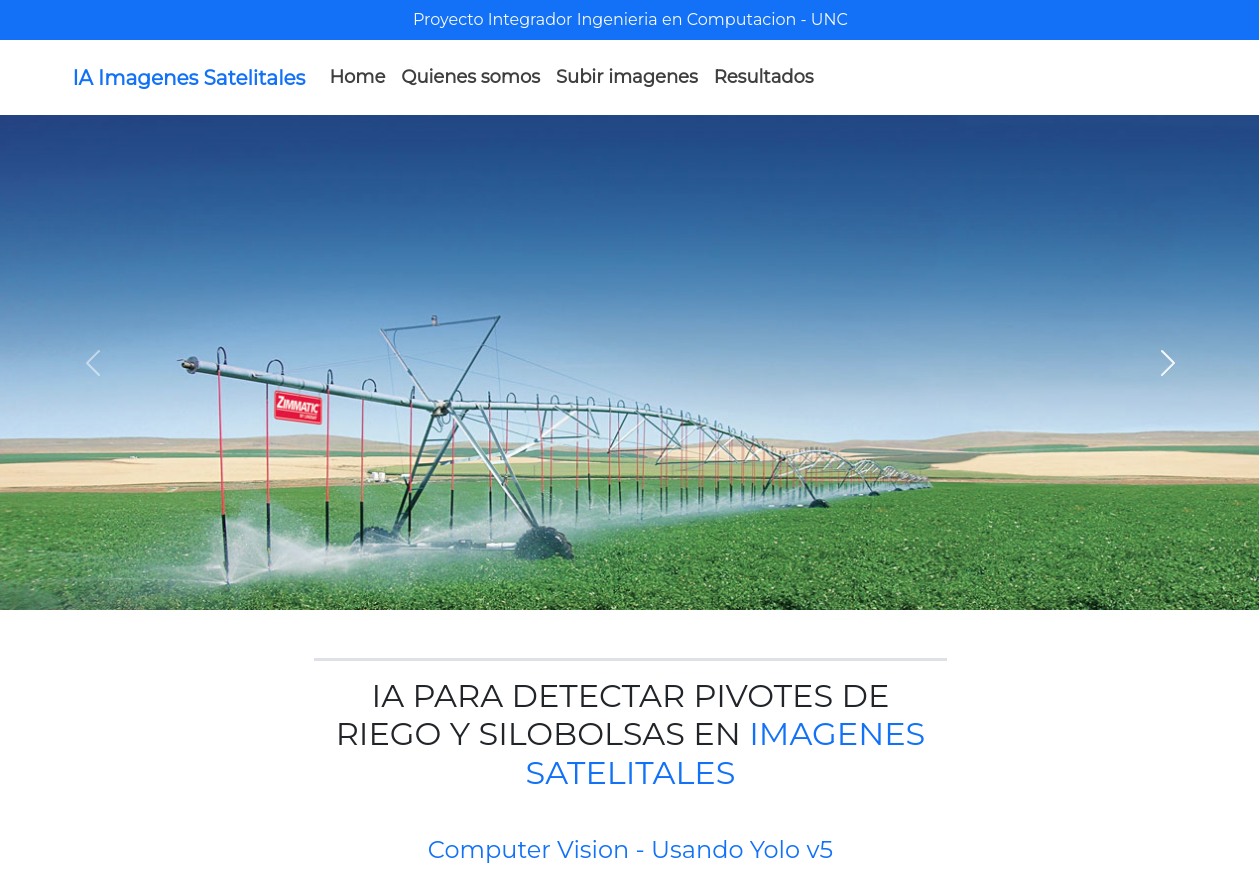
\includegraphics[width=1\textwidth]{img/FE - main.png}
    \caption{Página principal}
    \label{fig:main}
\end{figure}

\begin{figure}[b!]
    \centering
    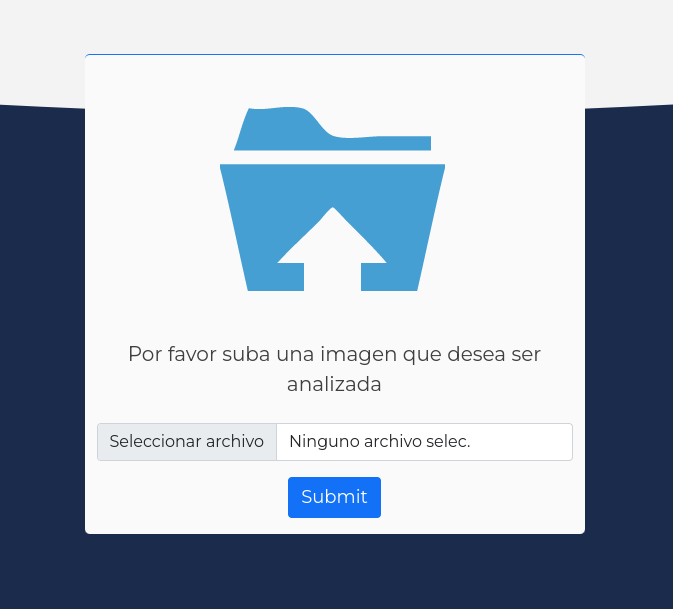
\includegraphics[width=0.6\textwidth]{img/FE - upload file.png}
    \caption{Subir una imagen para analizar}
    \label{fig:subir-imagen}
\end{figure}

\begin{figure}[h!]
    \centering
    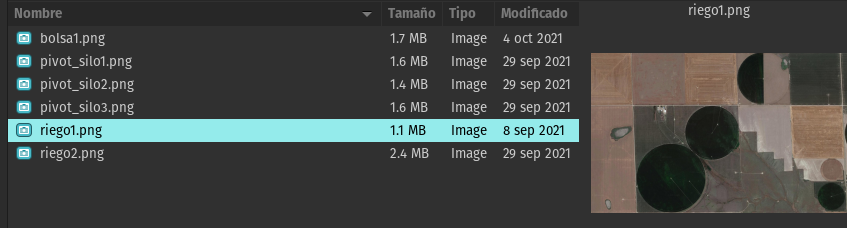
\includegraphics[width=1\textwidth]{img/FE - select file.png}
    \caption{Seleccionar una imagen desde la PC-Usuario}
    \label{fig:select imagen}
\end{figure}

\hfill \break
\\

\begin{table}[h!]
    \begin{tabular}{ | p{3cm} |p{9cm}| }
        \hline
        \rowcolor[HTML]{d6d8ff}
        TC-02 & Validar la presencia de una imagen cargada correctamente.\\
        \hline
        Objetivo & Obtener información sobre la validez o invalidez de la imagen subida por el usuario.\\
        \hline
        Procedimiento & \begin{enumerate}
            \item El usuario debe dirigirse a la página y luego de subir una imagen debe observar si el formato es aceptado.
            \item Luego debe ver habilitado el botón ``Submit'' para dar inicio a la Detección. 
        \end{enumerate}
        \\
        \hline
        Resultados esperados & Éxito en la presencia de la imagen subida.- Figura \ref{fig:subir-imagen}, \ref{fig:select imagen} y \ref{fig:loading1}\\
        \hline
        Estado & APROBADO \\
        \hline
    \end{tabular}\\
    \caption{Caso de Prueba del Requerimiento de Usuario R-02}
    \label{pruebar2}
\end{table}

\hfill \break
\\

\begin{figure}[h!]
    \centering
    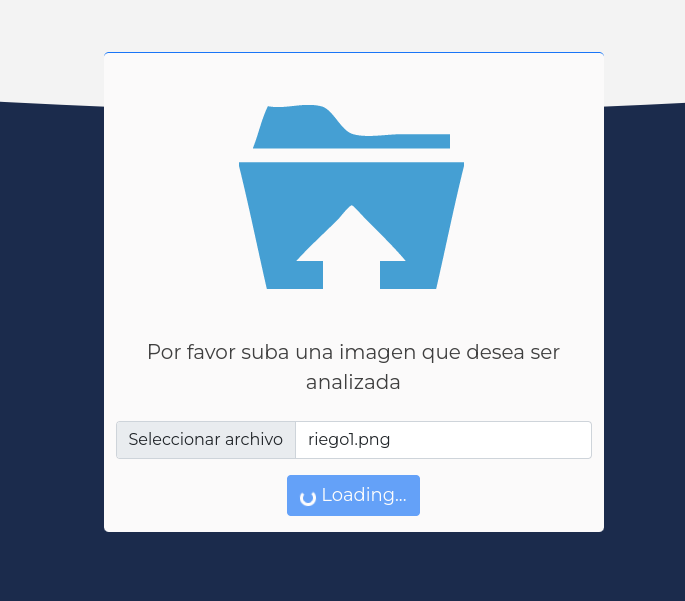
\includegraphics[width=0.6\textwidth]{img/FE - detection loading.png}
    \caption{Inicio de la detección - Loading}
    \label{fig:loading1}
\end{figure}

\begin{table}[h!]
    \begin{tabular}{ | p{3cm} |p{9cm}| }
        \hline
        \rowcolor[HTML]{d6d8ff}
        TC-03 & Validar cuando la imagen es de un formato erróneo, mostrar un mensaje del error y debe ser posible volver a cargar una nueva imagen.\\
        \hline
        Objetivo & Al obtener un mensaje sobre la invalidez de la imagen subida, volver a habilitar el botón para subir una nueva imagen.\\
        \hline
        Procedimiento & \begin{enumerate}
            \item El usuario debe dirigirse a la página y luego de subir una imagen errónea debe  observar un mensaje de imagen inválida.
            \item Luego debe ver habilitado el botón para volver a cargar una imagen nueva. 
        \end{enumerate}
        \\
        \hline
        Resultados esperados & Éxito en la presencia de un mensaje de formato inválido.- Figura \ref{fig:error1} muestra el mensaje de error. \\
        \hline
        Estado & APROBADO \\
        \hline
    \end{tabular}\\
    \caption{Caso de Prueba del Requerimiento de Usuario R-03}
    \label{pruebar3}
\end{table}

\begin{figure}[h!]
    \centering
    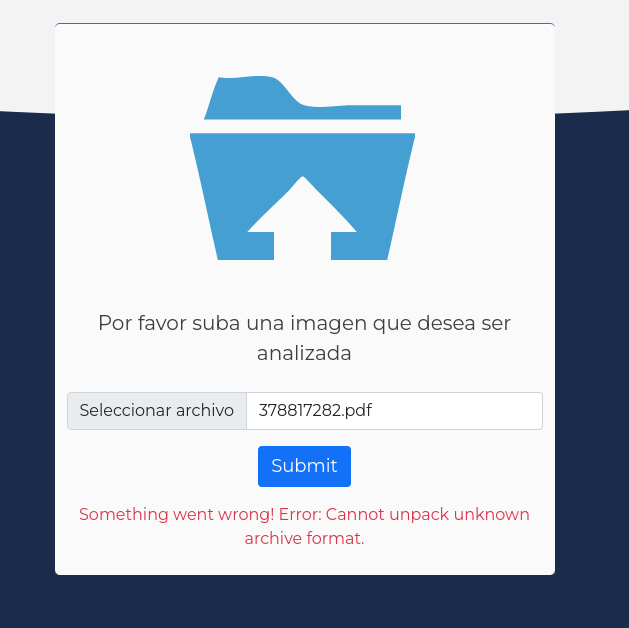
\includegraphics[width=0.6\textwidth]{img/FE - upload error.png} 
    \caption{Error al subir una archivo de formato invalido}
    \label{fig:error1}
\end{figure}


\begin{table}[h!]
    \begin{tabular}{ | p{3cm} |p{9cm}| }
        \hline
        \rowcolor[HTML]{d6d8ff}
        TC-04 & Validar que debe ser posible visualizar en la página la/s imágenes cargadas y un historial con información de las analizadas.\\
        \hline
        Objetivo & El usuario debe visualizar la información sobre todas las imágenes analizadas anteriormente y la actual.\\
        \hline
        Procedimiento & \begin{enumerate}
            \item El usuario debe dirigirse a la página, luego de subir/seleccionar una imagen y hacer clic en el botón de 'Submit', iniciará la detección automáticamente, 
            \item Luego, como resultado debe ver la imagen resultante con las detecciones encontradas.
            \item Además debe observar una tabla con el historial de todas las detecciones y los detalles de las mismas.
        \end{enumerate}
        \\
        \hline
        Resultados esperados & Éxito en la presencia de la imagen analizada y de una tabla con el historial de todas las imágenes analizadas hasta el momento.- Figuras \ref{fig:resultado} y \ref{fig:tabla result}.\\
        \hline
        Estado & APROBADO \\
        \hline
    \end{tabular}\\
    \caption{Caso de Prueba del Requerimiento de Usuario R-04}
    \label{pruebar4}
\end{table}

\begin{figure}[h!]
    \centering
    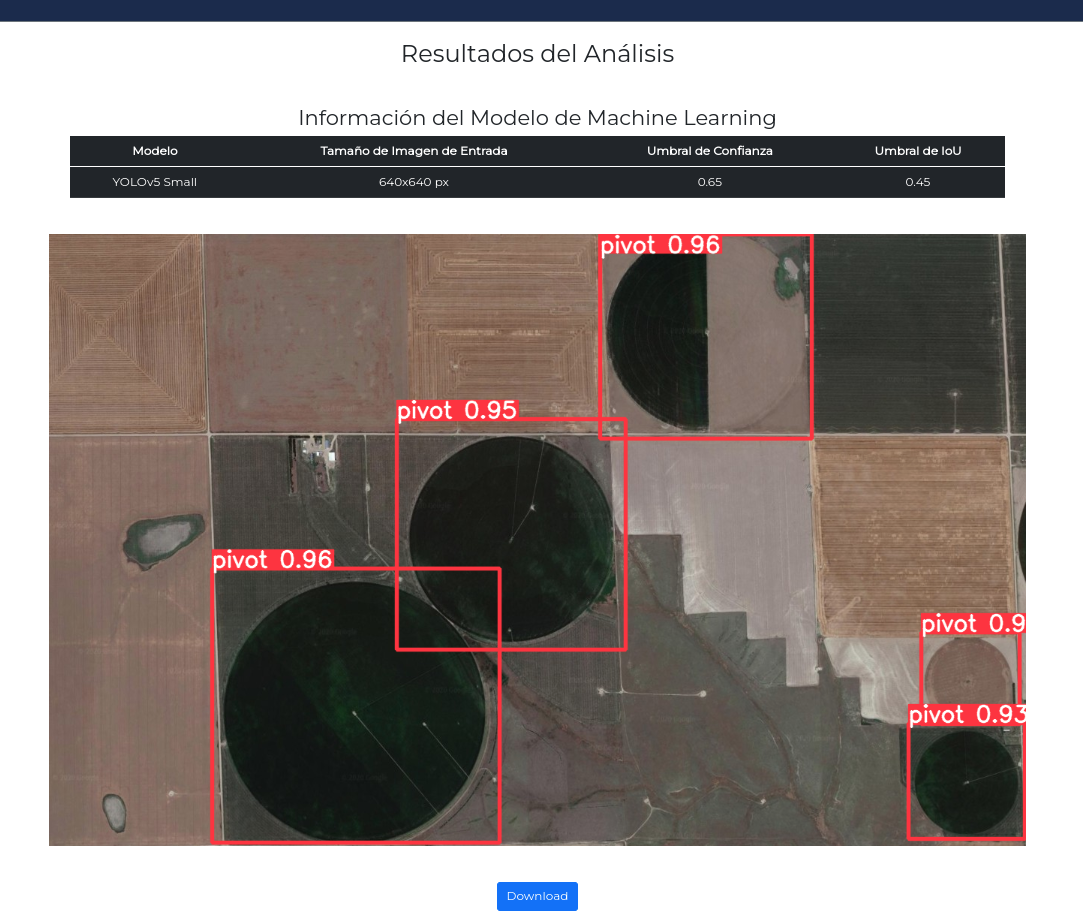
\includegraphics[width=0.92\textwidth]{img/FE - results.png}
    \caption{Fin de la detección - Resultado}
    \label{fig:resultado}
\end{figure}

\begin{figure}[h!]
    \centering
    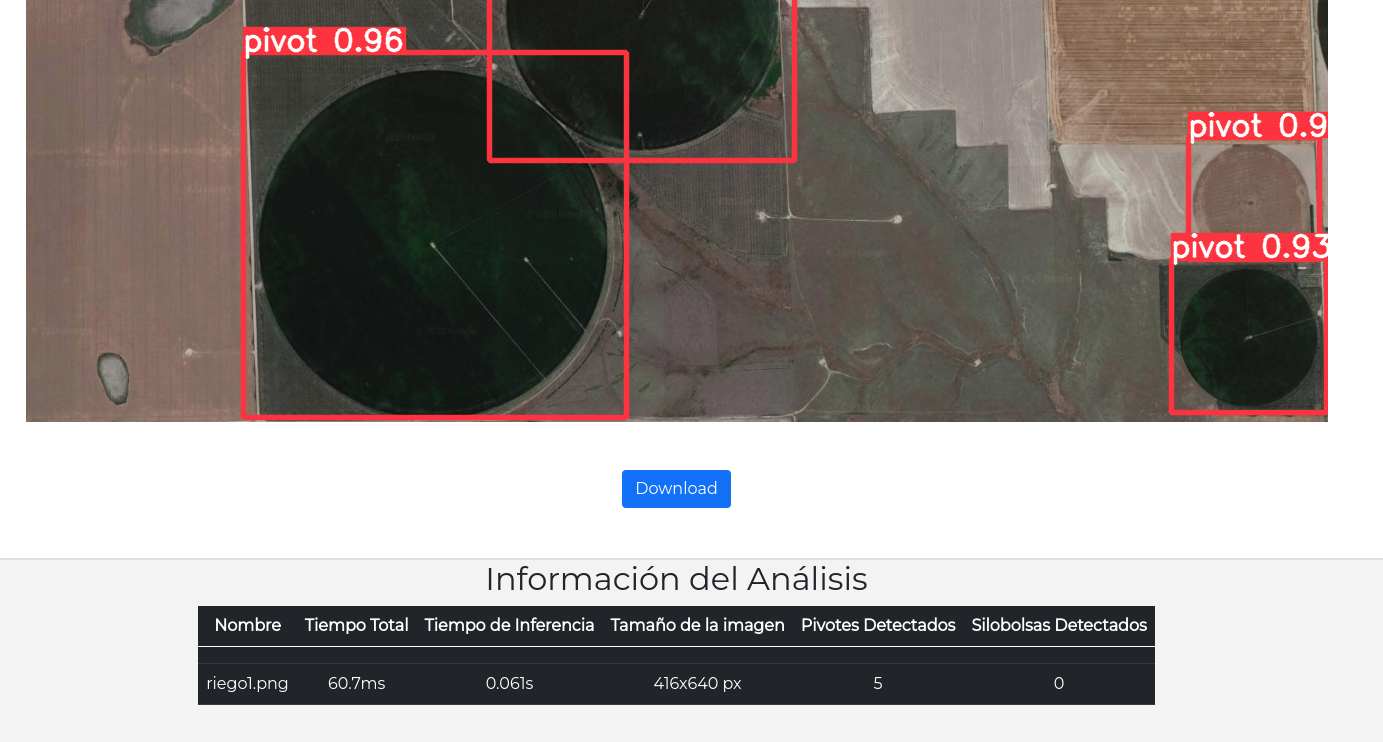
\includegraphics[width=1\textwidth]{img/FE - detection info table.png}
    \caption{Tabla de Información de detecciones - Resultado}
    \label{fig:tabla result}
\end{figure}

\hfill \break
\\

\begin{table}[h!]
    \begin{tabular}{ | p{3cm} |p{9cm}| }
        \hline
        \rowcolor[HTML]{d6d8ff}
        TC-05 & Validar que es posible analizar la imagen cargada, obtener información de la misma y que el sistema debe informar si se encontró algún objeto o no.\\
        \hline
        Objetivo & El usuario debe visualizar la imagen ya analizada y el resultado de la detección, remarcando donde se encuentran los objetos detectados y a que tipo corresponde: silobolsa o riego por pivote.\\
        \hline
        Procedimiento & \begin{enumerate}
            \item El usuario luego de solicitar que se analice una imagen, debe visualizar el resultado.
            \item La imagen resultante debe contener cuadros delimitadores encerrando a los objetos detectados e indicando su tipo.
        \end{enumerate}
        \\
        \hline
        Resultados esperados & Éxito en la presencia del resultado de la detección con información adicional .- Figura \ref{fig:bulk-detection} detalla el historial y los resultados de la detección. Figura \ref{fig:tabla result} muestra el resultado en caso de haber subido una sola imagen.\\
        \hline
        Estado & APROBADO \\
        \hline
    \end{tabular}\\
    \caption{Caso de Prueba del Requerimiento de Usuario R-05}
    \label{pruebar5}
\end{table}

\begin{figure}[h!]
    \centering
    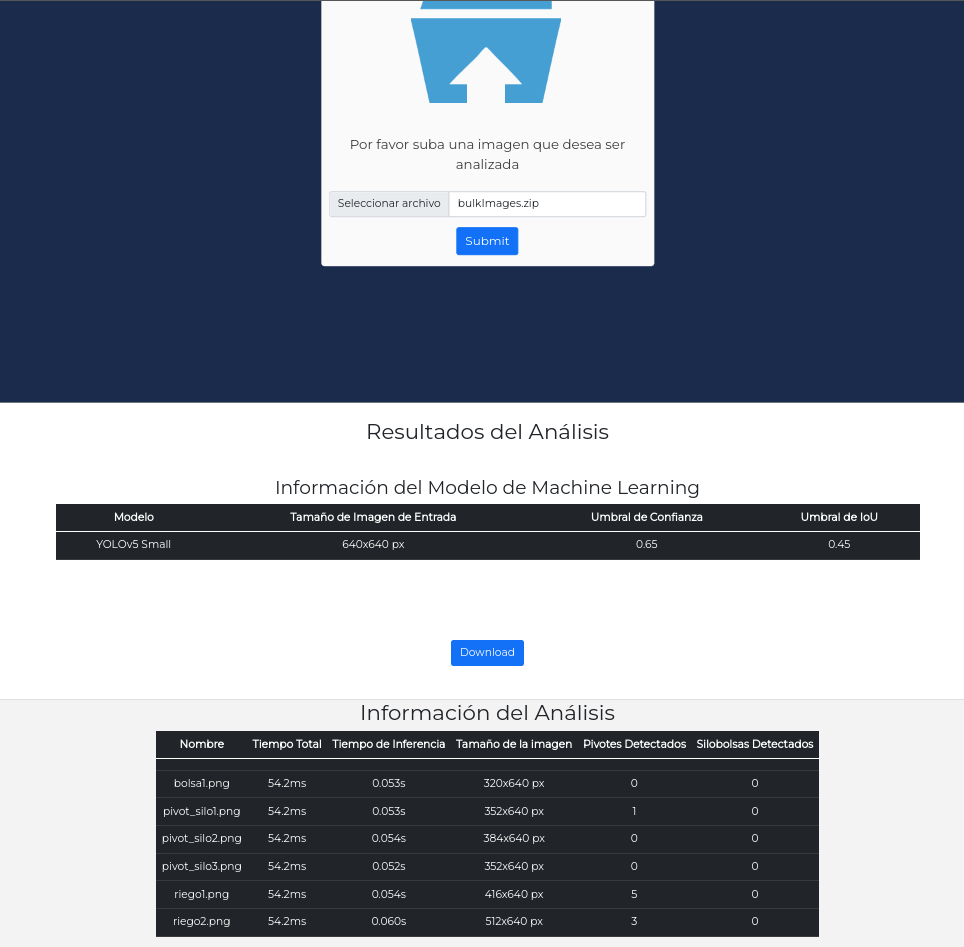
\includegraphics[width=0.93\textwidth]{img/FE - bulk detection.png}
    \caption{Detección de un archivo con imágenes comprimidas}
    \label{fig:bulk-detection}
\end{figure}

\hfill \break
\\

\hfill \break
\\

\begin{table}[h!]
    \begin{tabular}{ | p{3cm} |p{9cm}| }
        \hline
        \rowcolor[HTML]{d6d8ff}
        TC-06 & Validar que es posible descargar la imagen ya analizada.\\
        \hline
        Objetivo & El usuario debe poder visualizar y descargar la/s imagen/es analizada/s.\\
        \hline
        Procedimiento & \begin{enumerate}
            \item El usuario una vez que pueda visualizar la imagen analizada, debe tener la opción de descargarla a su máquina local.
            \item La imagen analizada y descargada debe encontrarse en la máquina local del usuario.
        \end{enumerate}
        \\
        \hline
        Resultados esperados & Éxito en la presencia de la imagen o un archivo con varias imágenes analizadas en la máquina local del usuario.-  Figura \ref{fig:download-file}.\\
        \hline
        Estado & APROBADO \\
        \hline
    \end{tabular}\\
    \caption{Caso de Prueba del Requerimiento de Usuario R-06}
    \label{pruebar6}
\end{table}

\begin{figure}[h!]
\centering
    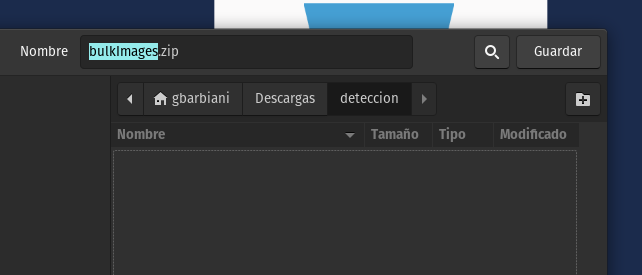
\includegraphics[width=1\textwidth]{img/FE - download file.png}
    \caption{Descarga de archivo con imágenes detectadas - Resultados}
    \label{fig:download-file}
\end{figure}

\hfill \break
\\

\newpage
\subsubsection{Matriz de trazabilidad}

En la matriz de trazabilidad presentada a continuación se relacionan todos los requerimientos planteados con los casos de test descritos en la sección anterior, con la finalidad de obtener una mejor visión general que todos los requerimientos fueron testeados exitosamente.

Los requerimientos no funcionales RNF-04 (Capacidad de ser desplegado fácilmente en diferentes sistemas) y RNF-05 (La API debe desarrollarse en Node.js y para la interfaz gráfica se debe usar CSS, HTML y JavaScript) no figuran en la matriz de trazabilidad, debido a que establecen metodologías y herramientas de trabajo.

\\
\begin{table}[h]
    \centering
    \begin{tabular}{ |p{2cm}|p{0.6cm} p{0.6cm} p{0.6cm} p{0.6cm} p{0.6cm}
                            |p{0.6cm} p{0.6cm} p{0.6cm} p{0.6cm} p{0.6cm} p{0.6cm}
                            |p{0.6cm} p{0.6cm} p{0.6cm} |  }
    
        \hline
          &\centering\rotatebox{90}{RF-AP1-01} &\centering\rotatebox{90}{RF-AP1-02} &\centering\rotatebox{90}{RF-AP1-03} &\centering\rotatebox{90}{RF-AP1-04} 
          &\centering\rotatebox{90}{RF-AP1-05} 
          &\centering\rotatebox{90}{RF-FE-01} &\centering\rotatebox{90}{RF-FE-02} &\centering \rotatebox{90}{RF-FE-03} &\centering \rotatebox{90}{RF-FE-04}      & \centering\rotatebox{90}{RF-FE-05}& \centering\rotatebox{90}{RF-FE-06}
          & \centering\rotatebox{90}{RNF-01} &\centering\rotatebox{90}{RNF-02} &\rotatebox{90}{RNF-03}\\
        \hline
        \centering{TC-01} & &\cellcolor[HTML]{D0F5A1}{\checkmark}& & & &\cellcolor[HTML]{D0F5A1}{\checkmark} &\cellcolor[HTML]{D0F5A1}{\checkmark} & & & & & &\cellcolor[HTML]{D0F5A1}{\checkmark}&\cellcolor[HTML]{D0F5A1}{\checkmark}\\
        \hline
        \centering{TC-02} &  &\cellcolor[HTML]{D0F5A1}{\checkmark}  & & & & &\cellcolor[HTML]{D0F5A1}{\checkmark} & & & & & & \cellcolor[HTML]{D0F5A1}{\checkmark} &\cellcolor[HTML]{D0F5A1}{\checkmark}\\
        \hline
        \centering{TC-03} & &\cellcolor[HTML]{D0F5A1}{\checkmark}   & & & & & \cellcolor[HTML]{D0F5A1}{\checkmark} & & & & & &\cellcolor[HTML]{D0F5A1}{\checkmark}  &\cellcolor[HTML]{D0F5A1}{\checkmark} \\
        \hline
        \centering{TC-04}&\cellcolor[HTML]{D0F5A1}{\checkmark} &\cellcolor[HTML]{D0F5A1}{\checkmark} &\cellcolor[HTML]{D0F5A1}{\checkmark} & &\cellcolor[HTML]{D0F5A1}{\checkmark} &\cellcolor[HTML]{D0F5A1}{\checkmark} &\cellcolor[HTML]{D0F5A1}{\checkmark} &\cellcolor[HTML]{D0F5A1}{\checkmark} &\cellcolor[HTML]{D0F5A1}{\checkmark} &\cellcolor[HTML]{D0F5A1}{\checkmark} & &\cellcolor[HTML]{D0F5A1}{\checkmark} &\cellcolor[HTML]{D0F5A1}{\checkmark}  &\cellcolor[HTML]{D0F5A1}{\checkmark}\\
        \hline
        \centering{TC-05}&\cellcolor[HTML]{D0F5A1}{\checkmark}& &\cellcolor[HTML]{D0F5A1}{\checkmark} & &\cellcolor[HTML]{D0F5A1}{\checkmark} &  & &\cellcolor[HTML]{D0F5A1}{\checkmark} &\cellcolor[HTML]{D0F5A1}{\checkmark} &\cellcolor[HTML]{D0F5A1}{\checkmark} & &\cellcolor[HTML]{D0F5A1}{\checkmark} &\cellcolor[HTML]{D0F5A1}{\checkmark}  &\\
        \hline
        \centering{TC-06} &\cellcolor[HTML]{D0F5A1}{\checkmark} & & &\cellcolor[HTML]{D0F5A1}{\checkmark} & &\cellcolor[HTML]{D0F5A1}{\checkmark} & &\cellcolor[HTML]{D0F5A1}{\checkmark} & & &\cellcolor[HTML]{D0F5A1}{\checkmark} & &\cellcolor[HTML]{D0F5A1}{\checkmark} & \\
        \hline
    \end{tabular}
    \caption{Matriz de Trazabilidad}
    \label{matriz}
\end{table}

\newpage

